% !TEX root = ../main.tex

\chapter{Background}\label{ch:background}
This chapter covers foundational concepts that will be discussed in the other chapters.

\section{Blockchain's Expanding Influence}
Blockchain is a decentralized, untrusted network wherein participants (nodes) can freely join or leave. There is no trusted central authority as all nodes work together with various consensus protocols, such as Proof of Work or Proof of Stake, to keep the integrity of data. In the case of hardware or communication failure of one node, other nodes continue to process requests seamlessly since each has a complete and consistent copy of data. The main features of blockchain are not restricted to technical resilience only. According to various reputable advisories~\cite{Gartner,Reportlinker}, blockchain has reached an average annual growth of 51\% from 2016 to 2022 and surpassing to more than \$2 billion USD in revenue by the year 2022. With the scope of blockchain applications to be further developed combined with the projected growth, blockchain will be one of the key technologies in less conservative industries.

The global blockchain market is expected to reach \$39.7 billion by 2025 with a annual growth rate of 67.3\%~\cite{GrandViewResearch2020}. Financial services are leading in adopting blockchain and all banks will be likely considering blockchain solutions in the near future for payment and settlement systems. Meanwhile, DeFi has been developing explosively by breaking the total value locked (TVL) of \$200 billion in 2021~\cite{MarketsandMarkets2020}. This demonstrates the ever-improving usability of blockchain for lending, borrowing, and trading applications without depending on any intermediate parties.

Moreover, the utility of blockchain is also growing out of finance sector. By 2025, at about 55\% of all healthcare applications are expected to have blockchain integrated in securing patient records~\cite{XcubeLabs2020}. Another fastest-adopting industry for blockchain is supply chain management to introduce more transparency and traceability. Large companies such as Walmart and IBM have already implemented blockchain mechanism in tracking products from their origins to retail~\cite{Sristy2021}.

\section{Ethereum's Smart Contract Ecosystem}
Out of 22 various implementations of the blockchain~\cite{builtin2024}, Ethereum~\cite{EIP150} is more widely accepted by the industry. It is a public blockchain proposed in 2013, deployed in 2015, and has the second largest market cap at the time of writing. It has a large development community which track enhancements and propose new ideas~\cite{CoinDesk20}. Ethereum enables decentralized applications to be deployed and executed on top of the blockchain. Smart contracts are essential component of the Ethereum and has been adopted widely by holding millions dollars worth of digital coins in form of ETH, ERC-20 tokens, Digital wallets and DeFi protocols.

Smart contracts are programs which get executed on the blockchain in a decentralized manner. Their conditions of execution lie inherently inside the code, which in return maintains some predefined rules. Smart contracts perform tasks on their own without the interference of any third-party intermediary. This gives more transparency in the contract operations with little risk of manipulation. Within the Ethereum ecosystem, smart contracts are deployed on-chain and, once published, become immutable and tamper-proof. They can be written by developers in any of Ethereum's high-level programming languages, such as Solidity and Vyper. Smart contracts can also handle simple token transfers to most complex dApps. Their programmability enables developers to define various kinds of interactions like token exchange, voting mechanism, or multi-signature wallets. Smart contracts are in fact the backbone of Ethereum functionality.

Like other emerging technologies, security is an important aspect of smart contracts. Previous research discovered that at about 45\% of existing smart contracts on the Ethereum are vulnerable~\cite{SmartContractSecurity}. The development of smart contracts has been proven to be error-prone, and as a result, smart contracts are often riddled with security vulnerabilities. One of the major smart contract hacks was due to TheDAO bug, which caused a loss of 60 million US dollars in June 2016~\cite{TheDAOCoinDesk}. Similar to other programming languages, smart contracts' codes can be exploited by an adversary (\ie Miner, external users and other contracts) to manipulate executions and gain profit. Some smart contracts have kept millions of dollars, which could be enough to incentivize adversaries to exploit vulnerabilities.

\begin{example}
	Aave is a decentralized lending protocol, with a total value locked (TVL) consistently exceeding \$6 billion. Users can earn interest by supplying assets or take out loans by borrowing crypto with their deposits as collateral. As another example, Uniswap, one of the largest decentralized exchanges (DEX), has a TVL of approximately \$3.7 billion and allows users to trade directly from their wallets~\cite{theblock2024}.
\end{example}

\section{Decentralized Apps and ERC-20 Tokens}
Migrating applications from centralized to decentralized architecture can solve many issues such as single point of failure, hardware and maintenance costs, and data security. This type of application is distributed over an untrusted network and leverage smart contracts to run codes on the blockchain. Tokens are subset of smart contracts and security is particularly important given that many tokens have considerable market capitalization. As tokens can be held by commercial firms, in addition to individuals, and firms need audited financial statements in certain circumstances, the correctness of the smart contract issuing the tokens is now in the purview of professional auditors.

Ethereum allows dApps to accept and use ETH as its protocol-level cryptocurrency or issue their own custom tokens with a variety of intents (\eg In-app purchase, Interoperability with other dApps, Representing digital assets, \etc). Tokens might be currencies with different properties than ETH, they may be required for access to a dApp's functionality or they might represent ownership of some off-blockchain asset. It is beneficial to have interoperable tokens with other dApps and off-blockchain webapps, such as exchange services that allow tokens to be traded. In this regard, the Ethereum community accepted a popular token standard called ERC-20~\cite{Interface}. As shown in Figure \ref{fig:interface}, ERC-20 is an interface that defines abstract methods (name, parameters, return types) and provides guidelines on how the methods should be implemented, however it does not provide an actual concrete implementation. Developers have the flexibility of implementing ERC-20 methods according to the needs of their dApps, or even expand it to offer new functionalities.

\begin{figure}[t]
	\centering
	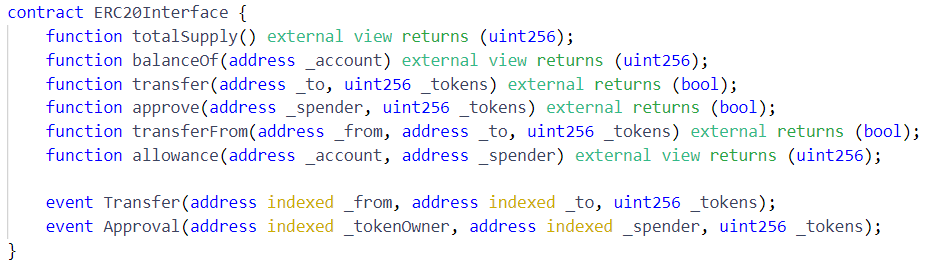
\includegraphics[width=\textwidth,keepaspectratio]{interface.png}
	\caption[The ERC-20 interface in Solidity]{The ERC-20 interface in Solidity defines a set of functions that any contract implementing the ERC-20 standard must include. These functions ensure interoperability and compatibility with other ERC-20 compliant contracts, wallets, exchanges, and decentralized applications.}
	\label{fig:interface}
\end{figure}

While numerous ERC-20 extensions or replacements have been proposed (\eg ERC-721, ERC-777, ERC-1155, \etc), ERC-20 remains prominent. Of the 2.5M smart contracts on the Ethereum network, 260K are tokens~\cite{TokenTracker}. 98\% of these tokens are ERC-20 tokens~\cite{TokenTracker}, demonstrating their widespread acceptance by the industry, smart contract developers and the Ethereum community. As shown in Figure \ref{fig:layers}, among the layers of the Ethereum blockchain, ERC-20 tokens fall under the \textit{Contract layer} in which back-end of DApps are executed.

\begin{figure}[t]
	\centering
	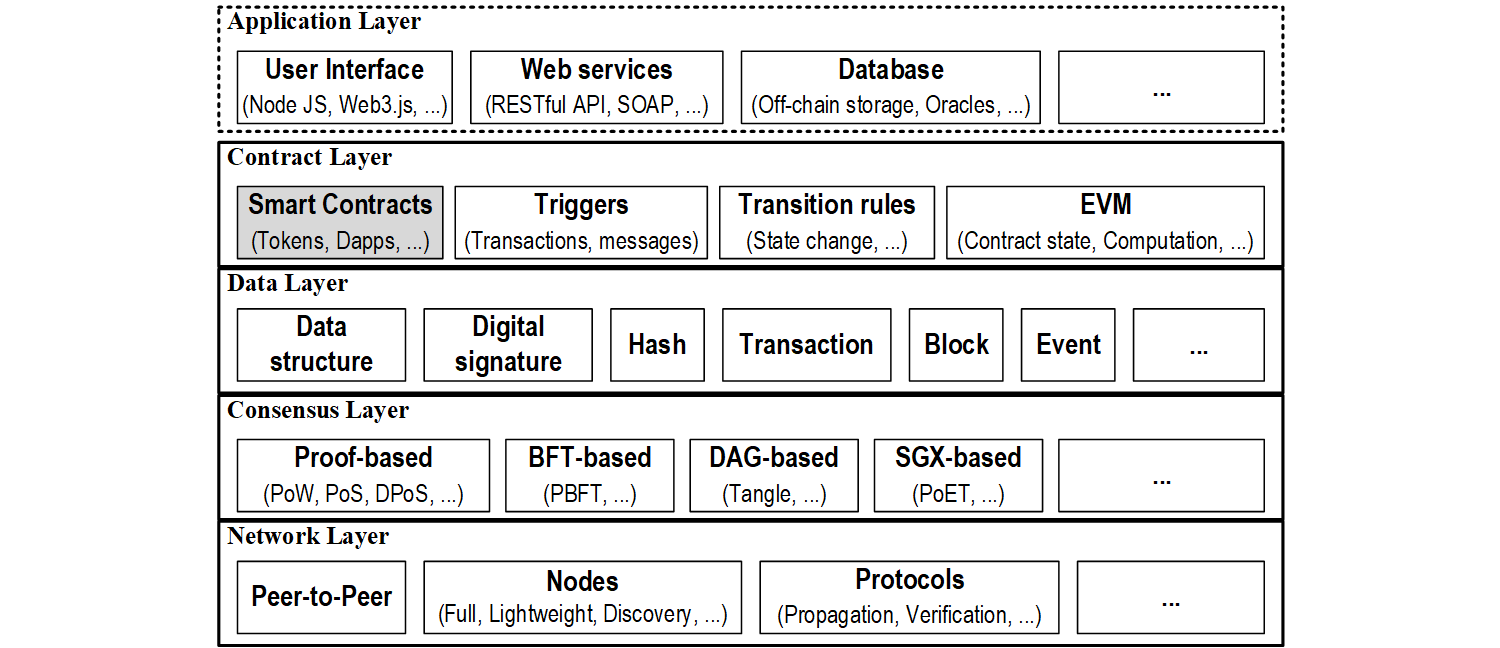
\includegraphics[width=0.8\textwidth,keepaspectratio]{blockchain.png}
	\caption[Ethereum layers and Smart Contract execution]{Smart contracts generally exist at the contract layer, leveraging the underlying consensus mechanisms for secure execution and state changes. The \textit{Contract Layer} can be considered a sub-layer of the \textit{Application Layer}, focusing on how smart contracts execute and interact with blockchain transactions.}
	\label{fig:layers}
\end{figure}

\section{Complexity of Leveraged Tokens}
\subsection{Models and Dynamic}
A typical Exchange-Traded Fund (ETF) is a weighted basket of stocks from firms with a common characteristic (\eg they all operate in a specific sector or have a high market capitalization). The issuer splits the basket into shares, which are bought and sold on exchanges just like individual stocks~\cite{liebi2020effect}.
\begin{example}
	One of the most traded ETFs is the \textsl{SPDR S\&P500 ETF} with ticker symbol \textsl{SPY}. It is issued by SSGA\anote{ssga} and holds a basket of stocks from nearly 500 publicly traded companies that are part of the S\&P500\anote{SP500} index. The S\&P500 index has globally served as a gauge for the performance of the U.S. stock market as a whole, due to its depth and diversity. Since SPY tracks the S\&P500 index, investors can gain broad exposure and diversify their investment risk across the stock performance of 500 companies in 11 sectors without the logistics or starting capital required to buy shares in all these companies.
\end{example}

Leveraged ETFs (LETFs) were introduced in 2006 and are ETFs designed to amplify the daily performance of the underlying basket (more on leverage in Section \ref{subsec:leveragedproduct}).\anote{underlying} Inverse LETFs aim to achieve a return that is a multiple of the inverse of the underlying asset’s daily performance~\cite{hill2009understanding,cheng2009dynamics,SEC}. Many investors alternatively refer to LETFs and inverse LETFs as ``Bullish'' and ``Bearish'' LETFs, respectively, reflecting their short-term sentiment on future price movements.
\begin{example}
	\textsl{Direxion Daily S\&P500 Bull 3x ETF (SPXL)} is a 3x (three times) LETF that seeks to deliver triple the daily performance of the S\&P500. It magnifies each 1\% gain in the S\&P500 index into a 3\% gain and loses 3\% for every 1\% drop in the index. \textsl{Direxion Daily S\&P500 Bear 3x ETF (SPXS)} delivers triple the opposite daily performance of the S\&P500 index. If the S\&P500 index depreciates by 1\%, SPXS gains 3\%, and vice versa~\cite{wided2019properties,lettau2018exchange}.
\end{example}

The equivalent of an LETF in the cryptocurrency and crypto-asset (``crypto'') market could be thought of as Leveraged Token (LVT). Similar to LETFs, LVTs use leveraged products offered in the crypto market to outperform the underlying asset’s return on a daily basis. While the majority of LETFs are actively managed funds\anote{active}, LVTs employ one of three management models: (i) centralized, (ii) decentralized, and (iii) hybrid. 

Centralized LVTs are mainly managed by crypto exchanges. They can be purchased on the spot market (similar to cryptocurrency) or directly from the issuer. Decentralized LVTs operate on the blockchain through smart contracts and can be traded without relying on a third-party. Hybrid LVTs are basically decentralized LVTs that are traded on centralized crypto exchanges. Users prefer centralized exchanges for their user-friendly interfaces, continuous-time order books (rather than automated market makers, which are the only trading mechanism efficient enough to run on-chain), and increased liquidity due to aggregated buy and sell orders.\anote{liquidity} However, this model introduces certain disadvantages resulting from the combination of centralized and decentralized systems (\eg functional complexities, security concerns, custodial risks, \etc.).

\begin{example}
	An issuer may offer BTC3L/BTC3S as a pair of LVTs tracking Bitcoin (BTC) as the underlying asset. A Bitcoin futures contract (BTC-Perp\anote{btc-perp}) can be used as the leveraged product to outperform Bitcoin in the short term. The number three in the LVT name represents the multiplier (triple-leveraged), while L/S stands for going long/short on the market.\anote{long-short} BTC3L gains 3\% when the price of Bitcoin rises by 1\%, and loses 3\% for every 1\% price drop. Conversely, when Bitcoin drops by 1\%, BTC3S gains 3\%, and loses 3\% for every 1\% price rise.
\end{example}

\subsection{Volatility Drag}\label{appx:voldrag}
Volatility can be defined as the rate of variation in values of a particular asset. A high volatility asset's value can be spread out over a bigger range of value and may change dramatically either way in a very short period of time. In contrast, the price of a low-volatility asset does not vary much and mostly remains constant. An example could be that, in the equity market, whenever the price of any particular stock has been continuously moved up or down by less than 1\%, for some considerable period of time. It is thought to be a volatile stock, especially when it passes this 1\% range compared to historical price~\cite{Investo_Volatility}.

\textsl{Volatility drag} represents the rate at which the value of investments dissipates\anote{vol-drag}. As volatility increases and positions are held for a longer period, the drag imposed by volatility accelerates, making it more destructive to the  value of the investment~\cite{tsalikis2019can,SeekingAlpha_Volatility}. A similar effect occurs in LVTs, which impacts the return.

\ExecuteMetaData[sections/tables]{tab-voldrag}

\begin{example}
	The performance of 3x and 5x Long/Short BTC tokens with a \$200 initial investment is compared in a volatile market. The assumption in Table \ref{tab:voldrag} is a 5\% BTC price increase on day 1, followed by another 5\% increase on day 2, and then a 10\% drop on day 3, continuing in this pattern. Mathematically, two 5\% increases on days 1 and 2 should be offset by a 10\% drop on day 3. However, the math does not align as expected due to accumulated profit or loss. The price of a non-leveraged BTC position increases by 5\% from \$200 to \$210 on day 1 and by another 5\% from \$210 to \$220.5 on day 2 (a 10.25\% gain after 2 days). A 10\% drop on day 3 from \$220.5 to \$198.45 results in a position that is -0.78\% lower than the initial investment, making the overall return negative. 
	
	This loss is -7.43\% and -21.88\% of the initial investment for BTC3L and BTC5L, respectively. Investors would expect better performance from BTC3S and BTC5S on the short side. However, due to accumulated losses in the first two days, they close at -6.08\% and -15.63\% lower than the starting value. Even after a week, when the initial investment has nearly reached the break-even point, all LVTs remain negative regardless of their leverage and direction (See Figure \ref{fig:voldrag}).
	
	\begin{figure}[t]
		\centering
		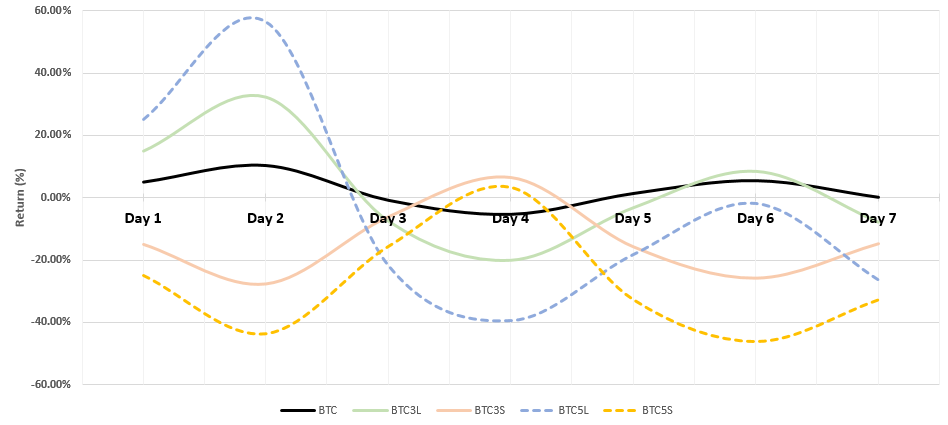
\includegraphics[width=0.9\textwidth,keepaspectratio]{voldrag.png}
		\caption[Volatility drag effect in volatile market]{LVT returns during a volatile week: the value of the initial investment (BTC in black) reached the breakeven point on day 7, but the returns of all LVTs remained negative due to the impact of volatility drag.}
		\label{fig:voldrag}
	\end{figure}
\end{example}

As the above example suggests, volatility negatively impacts the performance of LVT investments over time, as previously discussed in the case of LETFs~\cite{giese2010performance, trainor2011daily}. While volatility can be beneficial in the short term, compounded daily returns produce unexpected mathematical outcomes. Investors would have made some profits if they had closed their positions on the first or second day, but holding the position through the third day would have resulted in a loss. To minimize the impact of volatility drag on LVTs, it is better to use them as short-term investments in markets with strong trends and momentum.

\subsection{Leverage Products}
LVTs derive their value from a leveraged fund, which in turn is based on a leveraged product. This leveraged product usually originates from either the \textit{Crypto derivatives market} or the \textit{DeFi lending market} as highlighted in Figure \ref{fig:markets}. In the \textit{derivatives market}, Perpetual futures (Perps)\anote{perps} have become rather popular due to their flexibility. Because Perps do not expire, they can be held forever, with the additional advantage of being able to make leveraged positions in LVTs without any risk of contract expiration or rollover.

On the other hand, \textit{DeFi lending market} represents a more conservative alternative. It proposes the ability for LVTs to borrow assets through decentralized platforms like Aave and Compound.\anote{lending} Perpetual futures allow for higher leverage and are more riskier, while lending protocols provide lower leverage with reduced risk. In general, a choice between perpetual futures and lending protocols in the operation of LVTs depends on (i) specific design and purpose of the token, (ii) token's risk factor, (iii) the depth of liquidity provided by the underlying platform and (iv) the investment time horizon (short-term or long-term).

\begin{figure}[t]
	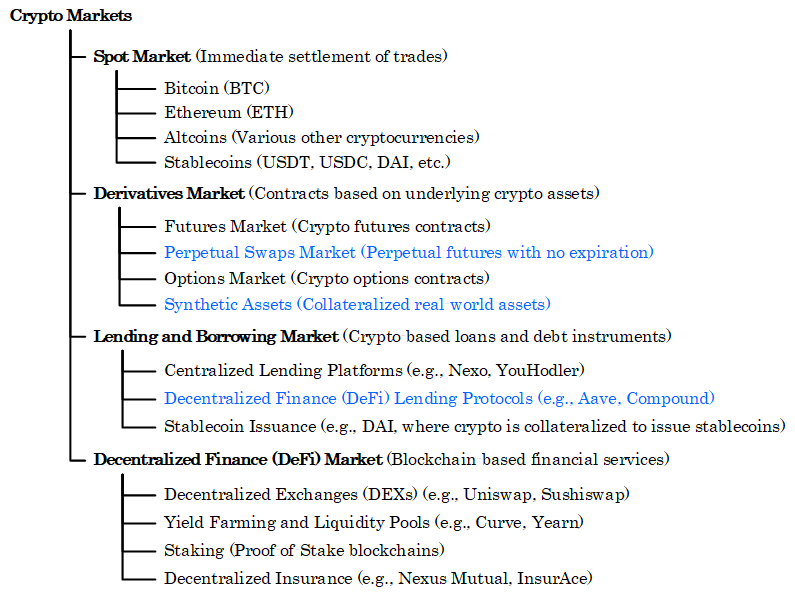
\includegraphics[width=\textwidth,keepaspectratio]{markets.png}
	\caption[Crypto market hierarchy]{A hierarchy of various types of crypto markets and instruments, delineates the positions of the Futures and Lending markets (in blue).}
	\label{fig:markets}
\end{figure}

LVTs essentially abstract away the hassle of maintaining a leveraged position for their users. They simplify management of such a position without requiring users to constantly monitor and manage margin requirements. But how do these LVTs actually generate the leverage on behalf of users? Both crypto derivatives and DeFi lending markets provide efficient ways to obtain desired leverage factors for LVTs. With relatively modest leverage ratio in LVTs-commonly up to 5x-one could be used to obtain leverage in either market. Leverage is typically generated by using dated futures, perpetual contracts, or synthetic assets in derivatives markets. In the DeFi lending market, leverage comes from the ability of borrowing funds and posting collateral. Reinvesting borrowed amount can increase exposure and generate leverage for LVTs (see the highlighted options in Figure \ref{fig:markets}). 

\subsubsection{Dated Futures}
They can be used in LVTs to provide leverage till specific expiration date.\anote{dated} Unlike perpetual futures, which have no expiration date, dated futures contracts require the position to be settled or rolled over by the expiration date. LVTs using dated futures must roll over contracts before their expiration date to maintain the leveraged exposure. The smart contract managing the LVT sells the expiring contracts and simultaneously buys new contracts with a later expiration date. This process ensures that the fund continues to maintain its leveraged exposure to the underlying asset without interruption. 

The rollover process can sometimes result in minor expenses or discrepancies in the leverage ratio, depending on the difference between the price of the expiring and new contract, referred to as the ``roll yield''. When the futures market is in Contango\anote{contango}, the roll yield is negative, and the LVT pays a premium to maintain its leveraged positions. In Backwardation\anote{backwardation}, the roll yield is positive, and the LVT benefits from the lower price of the new contract. Another risk is that the smart contract may fail to call the renewal or roll over process of the expired futures. This leads to a few consequences, including loss of leverage exposure, token devaluation, and possible liquidation in DEXs if holders rush to sell off the under-collateralized tokens.

\subsubsection{Perpetual Futures}
They can be utilized as leveraged products in LVTs without the need to roll over an expiring contract on a particular date in the future. This reduces slippage and costs associated with dated futures. However, perpetual futures impose funding fees as opposed to dated futures (see section \ref{appx:funding} for more information). Another disadvantage of them is that they are highly sensitive to volatility in the market. During big market swings, maintenance margin can rapidly change which increases the risk of forced liquidation. This makes perpetual futures more appropriate for short-term investment compared to buy-and-hold use cases.

\subsubsection{Automated Stacking}\label{appx:looping}
Looped positions (\ie borrowing, re-depositing, and borrowing again) on fixed-rate\anote{fixed} lending markets can be seen as somewhat analogous to dated futures contracts. Comparatively, variable-rate\anote{dynamic} positions on lending markets can be interpreted as the funding rate of the position, which in turn can be seen as a perpetual futures.

\subsubsection{Synthetic Assets}
These assets allow users to get exposure to a variety of asset price movements without necessarily owning them. Synthetic assets that track the value of fiat currencies, stocks, commodities, cryptocurrencies, and other financial derivatives already exist. They are usually backed by collateral (often in crypto) to ensure they maintain their value. For example, Synthetix protocol use collateralized debt to mint synthetic assets. They enable users to create tokens that track the value of real-world assets.

\subsubsection{Summary of Key Differences}\label{appx:summary}
An LVT is primarily utilized by investors who need a tokenized fund to simplify the management of leveraged positions with liquidation protection. Hence, identification of the target user becomes critical when choosing the right leveraged product before the issuance of LVTs. For the case of long-term investors, normally the debt market is cost-effective due to less daily depreciation of tokens. As described below, the futures are suitable for short-term investors.

\begin{itemize}
	\item \textit{Perpetual futures:} Best used for short-term leveraged tokens, which need rebalancing quite often. The positive feature of these tokens is their flexibility and the possibility of high leverage in both the short and long directions.
	
	\item \textit{Debt-based leveraged positions:} This strategy is more suitable for stable or conservative LVTs. However, it comes with the risks of liquidation and interest rate fluctuation. The maximum leverage is also constrained by the load-to-debt (LTV) ratio set by lenders and differs among blockchains. Besides, creating LVTs with short position is more challenging compared with long positions since overcollateralization is necessary (see the process of generating a short token in Figure \ref{fig:looping}).
	
	\item \textit{Synthetic assets:} Synthetic assets give leveraged exposure completely decentralized, but at the risk of overcollateralization and concerns of oracle accuracy. These characteristics make them less attractive to be used in LVTs.
\end{itemize}
Advantages and disadvantages of each leveraged product over key factors vary based on different investment horizons and issuer's preference. The main purpose of using LVTs is by the short-term traders who try to realize a profit in the same trading day. Therefore, perpetual futures shall be the most suitable to be utilized in LVTs. However, a debt-based LVT with different characteristics, which will be explained in the following chapters, may be suitable for issuers with long-term investment horizons.

\subsection{Key Factors in Crypto Futures Market}\label{appx:futures}
A futures contract, as explained, is an agreement to buy or sell a cryptocurrency at a given price at some future date. The Crypto Futures Market is the place where these contracts are traded, and such trading allows profiting on crypto price movements. Futures often refers to a class of derivatives that are traded in a market with much use of leverage, enabling traders to increase their exposure with less initial capital. It also allows hedging and speculation on future price movements. Perpetual futures are one of the dominant kinds of contracts in this market as users can keep a leveraged position open with no expiration date. The risks associated with these group of derivatives are mostly confined to the \textsl{Funding Rate} and the event of \textsl{Liquidation}.

\subsubsection{Funding Fee}\label{appx:funding}
Traditional futures contracts have an expiration date known as the delivery date. Futures prices converge with the spot price on this date. Before that, the market can be in one of two conditions: Contango or Backwardation~\cite{cme2020contango}. When the market is in Contango, futures are traded at a premium to the spot price (\ie they are more expensive). When the market is in Backwardation, futures are traded at a discount to the spot price (\ie they are cheaper than the spot price)~\cite{abd2019contango}. Contango or Backwardation may occur due to shocks in supply or demand, carrying costs, geopolitical situations, pandemics, etc. Ultimately, traditional futures prices converge with the spot price by the delivery date (see Figure \ref{fig:fundingfee}).

\begin{figure}[t]
	\centering
	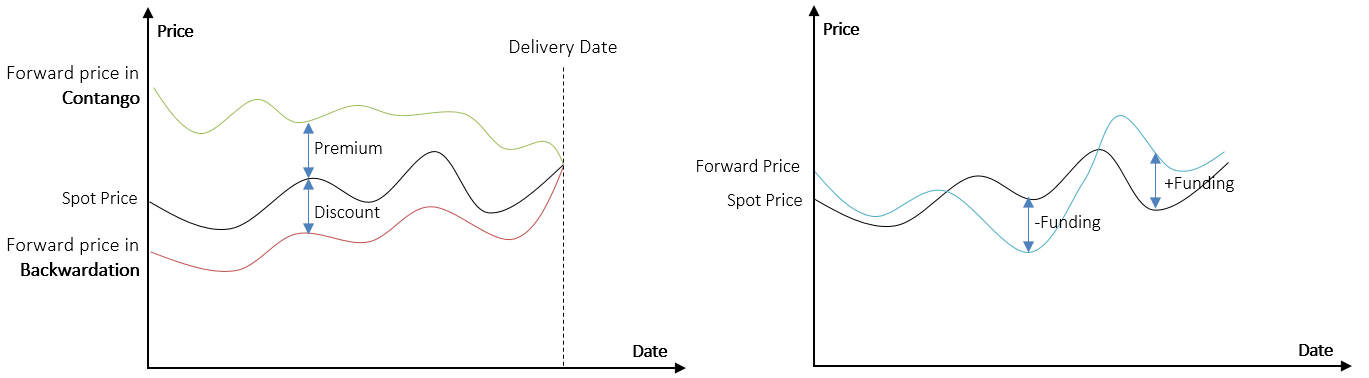
\includegraphics[width=\textwidth,keepaspectratio]{fundingfee.png}
	\caption[Price convergence in the Futures market vs. Perpetuals]{Contango or Backwardation conditions in the traditional futures market with a specific delivery date (left image). Price convergence over time in perpetual futures contracts, influenced by the funding rate (right image).}
	\label{fig:fundingfee}
\end{figure}

In crypto perpetual contracts, there is no delivery date, but the futures price still needs to settle against the spot price. At times, one side of the market becomes more aggressive, causing a disparity between spot and futures prices. To keep these prices aligned, a funding rate component is added to crypto futures. Only open positions are subject to funding payments or receipts at specific times (usually every 8 hours). If a position is closed before the funding exchange, traders do not pay or receive the funding fee. The funding fee can significantly impact high-leverage positions, potentially even leading to liquidation when paying for funding~\cite{Poloniex_FundingFee}.

Funding fee represents a periodic payment exchanged between traders holding long and short positions, intended to keep the contract's price (\(P_t\)) aligned with the underlying asset's spot price (\(S_t\)). When \(P_t > S_t\), the perpetual contract is trading at a premium, typically indicating higher demand for long positions. Conversely, when \(P_t < S_t\), the contract is trading at a discount, suggesting higher demand for short positions. The funding fee is a mechanism designed to encourage traders to take the opposite position and correct the imbalance. Let \(F_t\) represent the funding rate at time \(t\) expressed by:
\begin{equation}\label{eq:funding1}
	F_t = \alpha \left( \frac{P_t - S_t}{S_t} \right) + \beta \left( r_f - r_c \right)
\end{equation}
where \( r_f \) denotes the interest rate of the fiat currency and \( r_c \) denotes the interest rate of the cryptocurrency. Subsequently, \((\frac{P_t - S_t}{S_t})\) and \((r_f - r_c)\) are the "premium or discount" and "interest rate" components, with weighted coefficients \( \alpha \) and \( \beta \), respectively. Both \( \alpha \) and \( \beta \) are adjustable parameters that exchanges or DeFi platforms might calibrate based on market conditions, volatility, and the desired level of price convergence between the perpetual contract and the spot market. For instance, a high \( \alpha \) might be used in a highly volatile market to quickly correct large premiums or discounts, while a high \( \beta \) might be more relevant in a market where the cost of capital (borrowing rates, staking yields, etc.) is highly volatile~\cite{Binance_Funding,BitMEX_Funding}.

\subsubsection{Liquidation}\label{subsec:liquidation}
It happens when the positions in futures are automatically closed because of an inability to maintain a margin. The main drivers for liquidation are:
\begin{itemize}
	\item \textsl{Adverse price movements:} The market moves against the position, which may lead to a decline in the notional value and reduced account equity.
	
	\item \textsl{Unfavorable funding rates:} Whenever the funding rate is negative for the position, it causes a constant drain from the initial margin balance. Over time, the funding payments erode the initial margin, dropping it below the maintenance margin level-usually 5-10\% of the initial margin. The exchange will then liquidate the position without user consent.
\end{itemize}
The liquidation process is triggered when the price of the underlying asset falls below the \textit{liquidation price}, at which the value of the initial margin is no longer adequate. The liquidation price ($P_{Liq}$) can be calculated as \(P_{Liq} = P_{Ent} \times \left( 1 - \frac{1 - \mu}{\lambda} \right)\), where \(\lambda\) represents the leverage of the position (negative for shorts), \(P_{Ent}\) is the entry price and \(\mu\) is maintenance margin in percentage.

\begin{example}\label{ex:funding2}
	Bob opens a 10x long BTC/USDT Perps at \(P_{Ent} = \$30K\) with an initial margin of \$3K and a maintenance margin of \(\mu = 5\%\). Since this is a 10x position (\(\lambda = 10\)), it requires 10 times less capital than the full position value. The liquidation price is calculated as \(P_{Liq} = \$30K \times ( 1 - \frac{1 - 5\%}{10} ) = \$30K \times 0.905 = \$27,150\), at which point Bob’s position would automatically be closed by the exchange, and his initial margin of \$3K would be used to cover the losses. In other words, Bob loses his entire initial investment as a result of liquidation.
\end{example}